% HELIX — IJCKG submission (Springer LNCS format)
% Compile:  pdflatex main  ->  bibtex main  ->  pdflatex main  ->  pdflatex main
\documentclass[runningheads]{llncs}

\usepackage[T1]{fontenc}
\usepackage{graphicx}
\usepackage{marvosym}   % \Letter = corresponding-author envelope symbol (the "(B)" mark)
\usepackage{booktabs}
\usepackage{amsmath}
\usepackage{amssymb}   % \checkmark in Table 1
\usepackage{xcolor}
\usepackage{listings}
\usepackage{tikz}
\usetikzlibrary{arrows.meta,positioning,shapes.geometric,fit,backgrounds,calc}
\usepackage{pgfplots}
\pgfplotsset{compat=1.18}
\usepackage{algorithm}
\usepackage{algpseudocode}
\usepackage[hidelinks]{hyperref}
\renewcommand\UrlFont{\color{blue}\rmfamily}

% ---- helpers for drafting -----------------------------------------------------
\newcommand{\todo}[1]{\textcolor{red}{\textbf{[TODO: #1]}}}
\newcommand{\result}[1]{\textcolor{blue!70!black}{\underline{#1}}} % illustrative placeholder number
\lstset{basicstyle=\ttfamily\footnotesize,breaklines=true,frame=single,
        columns=fullflexible,keepspaces=true}

\begin{document}

\title{\textbf{HELIX}: \textmd{\textbf{H}ybrid \textbf{E}ntity
       \textbf{L}inking with \textbf{I}nteractive
       e\textbf{X}pert-in-the-loop Annotation}}
\titlerunning{HELIX: Hybrid, Graph-Aware Entity Linking Annotation}

% \orcidID adds the ORCID icon/link next to the author (LNCS-supported).
\author{Lakshan Karunathilake(\Letter)\inst{1,2}\orcidID{0000-0002-5606-4244} \and
Hideaki Takeda\inst{2,1}\orcidID{0000-0002-2909-7163}}
\authorrunning{L. Karunathilake and H. Takeda}
\institute{The Graduate University for Advanced Studies (SOKENDAI),
Shonan Village, Hayama, Kanagawa 240-0193, Japan \and
National Institute of Informatics, 2-1-2 Hitotsubashi, Chiyoda-ku,
Tokyo 101-8430, Japan\\
\email{lakshan@nii.ac.jp}}

\maketitle

% ---- Abstract ----------------------------------------------------------------
\begin{abstract}
Linking entity mentions to canonical knowledge-base entries is central to
building structured biomedical resources, yet automated systems remain below the
precision that downstream use requires, leaving expert curation the bottleneck.
We present \emph{HELIX}, an open-source, configurable annotation tool that unites
dense candidate retrieval with knowledge-graph-aware human review in a single
expert-in-the-loop workflow over any FAISS-indexable knowledge base. Candidates are
retrieved by a domain-adapted dense encoder over the knowledge base. HELIX's
distinguishing contribution is a two-level, graph-aware annotation process that targets the
\emph{Acc@$k$--Acc@1 gap} --- cases where the gold concept is retrieved but not
ranked first --- using document-level graph coherence, while the expert can
accept or challenge every decision: at the
\emph{individual} level, each mention's candidates are shown with their
neighbourhood in a connected knowledge graph (Neo4j), so annotators disambiguate
by graph context rather than surface text; at the \emph{document} level, the
accepted entities are assembled into one subgraph, isolated picks are flagged for
renegotiation, and identifiers can be rearranged until the document's entity set
is globally coherent. We evaluate HELIX on both tracks of BC5CDR (MeSH) and on
MedMentions ST21pv (UMLS, $203{,}282$ mentions). BC5CDR figures are a favourable
in-dictionary ceiling (up to $96\%$), while the open-vocabulary MedMentions/UMLS
setting shows that dictionary \emph{coverage} dominates retrieval quality --- whole
semantic types fall to near-zero when they are absent from the index. We also
profile the Neo4j graph
step's cost (nodes tackled, edges discovered, and per-document query latency), and
report the automatic graph
connection-maximisation as a negative result that motivates confidence-gated,
interactive use, and release HELIX with a reproducible setup to support scalable
entity-linking annotation.

\keywords{Biomedical Entity Linking \and Knowledge Graphs \and
Human-in-the-Loop Annotation \and
Dense Retrieval \and Collective Disambiguation.}
\end{abstract}

% ==============================================================================
\section{Introduction}
\label{sec:intro}

Entity linking (EL) maps textual mentions to canonical entries in a knowledge
base (KB) such as the UMLS Metathesaurus~\cite{umls}, and is a prerequisite for
constructing biomedical knowledge graphs, normalising clinical text, and
enabling structured search. Despite steady progress, fully automated biomedical
EL still plateaus well below the precision required for curated resources: strong
systems on recent shared tasks report top-1 accuracy in the range of roughly
$0.7$~\cite{bionne,belb}. As a result, high-quality resource construction remains
a human-in-the-loop activity in which expert curators verify, correct, and
disambiguate system suggestions.

Two gaps make this curation harder than it needs to be. First,
candidates are typically presented as \emph{flat text cards}---an identifier, a
label, a few aliases---which strips away the relational structure that makes
disambiguation easy for a human (is this ``lung'' an anatomical structure or a
disease?). Second, EL is usually performed \emph{one mention at a time}, so
decisions that ought to cohere across a document---two mentions of the same
concept, or two related concepts---are made independently and can silently
conflict.

We address these gaps with \emph{HELIX}, a configurable, open-source
expert-in-the-loop annotation tool. HELIX combines (i) dense candidate retrieval
over the knowledge base and (ii) a two-level, graph-aware review process backed by a
Neo4j knowledge graph. At the \emph{individual} level, the annotator sees each
mention's candidates together with their graph neighbourhood; at the
\emph{document} level, all accepted entities are drawn as one subgraph in which
isolated picks are flagged and can be renegotiated until the document is globally
coherent, turning independent per-mention choices into a human-driven collective
linking step.

\medskip\noindent\textbf{Contributions.}
\begin{enumerate}
  \item A \emph{dense retrieval} back end (a domain-adapted SAPBERT$+$FAISS
        encoder) that generates candidate concepts over any FAISS-indexable
        knowledge base (Sec.~\ref{sec:retrieval}).
  \item A \emph{two-level graph-aware annotation workflow} --- candidate-neighbourhood
        disambiguation and a document-level coherence-negotiation view --- with a
        \emph{confidence-gated} collective-linking algorithm that targets the
        Acc@$k$--Acc@1 gap without disturbing confident picks, and lets the
        expert challenge every decision (Sec.~\ref{sec:graph}).
  \item An \emph{open, reproducible system}---multi-select annotation, provenance
        logging, containerised deployment, and an evaluation harness---together
        with an empirical study on a biomedical corpus (Sec.~\ref{sec:eval}).
\end{enumerate}

% ==============================================================================
\section{Related Work}
\label{sec:related}

\subsubsection{Biomedical entity linking back ends.}
Neural biomedical EL is dominated by bi-encoder retrieval over synonym-rich
representations. BioSyn~\cite{biosyn} introduced synonym marginalisation, and
SAPBERT~\cite{sapbert} self-aligns biomedical entity representations against UMLS
synonymy, becoming the standard candidate generator. Lexical baselines such as
QuickUMLS~\cite{quickumls} and scispaCy~\cite{scispacy} remain fast and
training-free. Benchmarks such as BELB~\cite{belb} unify heterogeneous corpora and
KBs, and the BioNNE-L shared task~\cite{bionne} provides a multilingual evaluation
setting. HELIX uses a domain-adapted SAPBERT encoder as its candidate generator.

\subsubsection{Retrieval-and-rerank and LLMs for EL.}
The retrieve-and-rerank paradigm separates candidate generation from
disambiguation. Recent work applies LLMs to the reranking stage: retrieval-augmented
concept recognition~\cite{real}, constrained/contrastive decoding for biomedical
EL~\cite{llm4bioel}, generative re-ranking~\cite{belink}, alias-based retrieval
with LLM ranking for cross-lingual EL~\cite{bioelx}, and long-context,
document-consistent linking~\cite{longbel}. HELIX keeps the human in the loop and
takes this paradigm only as motivation for a future direction
(Sec.~\ref{sec:future}): \emph{automating} the grounded selection the annotator now
makes over the retrieved candidates, rather than issuing an autonomous prediction.

\subsubsection{Graph-based and collective disambiguation.}
A long line of work exploits KB structure for disambiguation, from topic-coherence
over semantic graphs~\cite{collective2020} and Personalized-PageRank collective
linking to entity-/relationship-embedding methods on knowledge
graphs~\cite{kgdisamb2021}. These systems infer coherence \emph{automatically};
HELIX instead \emph{surfaces} the graph neighbourhood to a human and makes the
document-level coherence check an interactive, auditable step---a
human-driven analogue of collective disambiguation.

\subsubsection{Annotation tools.}
General-purpose annotation platforms such as BRAT~\cite{brat} and
INCEpTION~\cite{inception} support entity and KB-linking annotation, and
INCEpTION adds machine assistance and active learning.
MedCATTrainer~\cite{medcattrainer} targets biomedical NER$+$L with active
learning. Evaluation and review tooling includes ELEVANT~\cite{elevant} for
fine-grained EL error analysis and AnNER~\cite{anner} for annotation/review
workflows in KG construction. Table~\ref{tab:tools} positions HELIX against these
tools: to our knowledge HELIX is the first annotation tool to combine dense
retrieval with a graph-neighbourhood/document-coherence review surface in one
workflow.

\begin{table}[t]
\caption{Feature comparison of HELIX with representative EL annotation tools.
\checkmark~= supported, $\circ$~= partial/plugin, --~= none. Columns: knowledge-base
\emph{link}ing, \emph{dense} retrieval, knowledge-graph \emph{neighbourhood} view,
\emph{document}-level coherence review, \emph{auto}-suggestion, \emph{provenance}
logging.}
\label{tab:tools}
\centering
\setlength{\tabcolsep}{5pt}
\footnotesize
\resizebox{\columnwidth}{!}{%
\begin{tabular}{lcccccc}
\toprule
Tool & Link & Dense & Graph & Doc. & Auto & Prov. \\
\midrule
BRAT~\cite{brat}                   & \checkmark & --         & -- & -- & --         & $\circ$ \\
INCEpTION~\cite{inception}         & \checkmark & $\circ$    & -- & -- & \checkmark & \checkmark \\
MedCATTrainer~\cite{medcattrainer} & \checkmark & \checkmark & -- & -- & \checkmark & \checkmark \\
Prodigy~\cite{prodigy}             & \checkmark & $\circ$    & -- & -- & \checkmark & \checkmark \\
\midrule
\textbf{HELIX (ours)}              & \checkmark & \checkmark & \checkmark & \checkmark & \checkmark & \checkmark \\
\bottomrule
\end{tabular}%
}
\end{table}

% ==============================================================================
\section{System Overview}
\label{sec:system}

HELIX structures entity-linking annotation as a pipeline of phases through which
each mention flows, keeping the human annotator in control at the review phases
(Fig.~\ref{fig:arch}): automated components \emph{propose}, and the annotator
\emph{disposes}. After a corpus is loaded as a session, HELIX
(1)~\emph{retrieves} candidate concepts for every mention from a knowledge base with
a domain-adapted dense encoder; (2)~presents each mention to the annotator for
\emph{individual review} in its document context, together with the ranked
candidates and their neighbourhood in a knowledge graph; and (3)~assembles the
accepted entities of a document for a \emph{coherence review}, where the annotator
renegotiates picks that are inconsistent with the
rest of the document. Every decision is persisted with its provenance. Each
automated component is optional and configurable per session, and the system is
domain-agnostic---it works with any concept inventory and, optionally, a companion
knowledge graph.

\begin{figure}[t]
\centering
\resizebox{\columnwidth}{!}{%
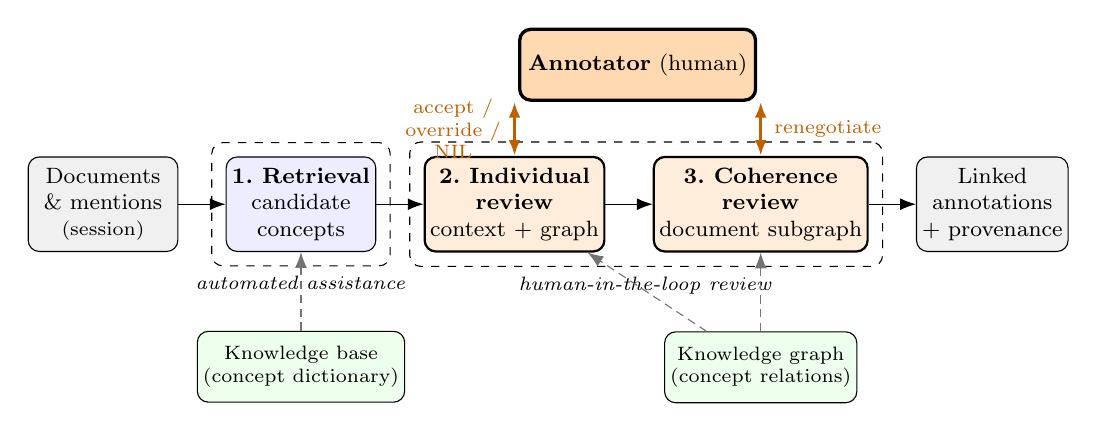
\begin{tikzpicture}[
  font=\footnotesize,
  phase/.style={draw,rounded corners,align=center,minimum height=12mm,
                minimum width=19mm,inner sep=2pt},
  auto/.style={phase,fill=blue!7},
  human/.style={phase,fill=orange!14,thick},
  io/.style={phase,fill=black!6},
  res/.style={draw,rounded corners,align=center,fill=green!7,
              font=\scriptsize,minimum height=9mm,minimum width=22mm,inner sep=2pt},
  actor/.style={draw,rounded corners,align=center,fill=orange!30,very thick,
                minimum height=9mm,inner sep=3pt},
  arr/.style={-{Latex[length=2mm]}},
  hitl/.style={{Latex[length=2mm]}-{Latex[length=2mm]},very thick,orange!75!black},
  feed/.style={-{Latex[length=2mm]},densely dashed,black!55}]

  % --- phase pipeline (left to right) ---
  \node[io]                       (inp)  {Documents\\\& mentions\\{\scriptsize(session)}};
  \node[auto,right=6mm of inp]    (ret)  {\textbf{1.\ Retrieval}\\candidate\\concepts};
  \node[human,right=6mm of ret]   (indiv){\textbf{2.\ Individual}\\\textbf{review}\\context $+$ graph};
  \node[human,right=6mm of indiv] (doc)  {\textbf{3.\ Coherence}\\\textbf{review}\\document subgraph};
  \node[io,right=6mm of doc]      (out)  {Linked\\annotations\\$+$ provenance};

  \draw[arr] (inp)--(ret);   \draw[arr] (ret)--(indiv);
  \draw[arr] (indiv)--(doc); \draw[arr] (doc)--(out);

  % --- human actor above the two review phases ---
  \node[actor,above=13mm of $(indiv)!0.5!(doc)$] (ann)
        {\textbf{Annotator} (human)};
  \draw[hitl] (ann.south-|indiv) -- node[left=1pt,font=\scriptsize,align=center]
        {accept /\\override /\\NIL} (indiv.north);
  \draw[hitl] (ann.south-|doc) -- node[right=1pt,font=\scriptsize,align=center]
        {renegotiate} (doc.north);

  % --- resources feeding the phases (below) ---
  \node[res,below=10mm of ret] (kb) {Knowledge base\\(concept dictionary)};
  \node[res,below=10mm of doc] (kg) {Knowledge graph\\(concept relations)};
  \draw[feed] (kb) -- (ret);
  \draw[feed] (kg) -- (indiv);
  \draw[feed] (kg) -- (doc);

  % --- phase-group backdrops ---
  \begin{scope}[on background layer]
    \node[draw,dashed,rounded corners,fit=(ret),inner sep=5pt,
          label={[font=\scriptsize]below:\emph{automated assistance}}]{};
    \node[draw,dashed,rounded corners,fit=(indiv)(doc),inner sep=5pt,
          label={[font=\scriptsize]below:\emph{human-in-the-loop review}}]{};
  \end{scope}
\end{tikzpicture}%
}
\caption{HELIX annotation flow. Automated \emph{retrieval} proposes candidates from a
knowledge base (blue); the annotator then performs \emph{individual review} (mention
in context, candidates, and their graph neighbourhood) and \emph{coherence review} of
the document subgraph, accepting, overriding, or renegotiating picks (orange). The
human controls the review phases (solid); a knowledge base and optional graph supply
candidates and relations (dashed).}
\label{fig:arch}
\end{figure}

% ------------------------------------------------------------------------------
\paragraph{Implementation and release.}
HELIX is a containerised client--server application --- web UI, API, a SAPBERT/FAISS
retrieval server, and Neo4j --- reproducible with a single command and configured via
version-controlled files; a utility converts UMLS \texttt{MRREL}/\texttt{MRCONSO} into
Neo4j bulk-import CSVs. Source, configuration, and the evaluation harness are
released.\footnote{\url{https://github.com/LakshanKarunathilake/HELIX}}

\subsection{Candidate Retrieval}
\label{sec:retrieval}

For a mention $m$, HELIX retrieves a ranked candidate list from a domain-adapted
dense encoder: SAPBERT~\cite{sapbert} embeddings (with a MeSH adapter) indexed
with FAISS~\cite{faiss} and scored by cosine similarity. The top candidates form
the grounded set that HELIX presents to the annotator. Retrieval is decoupled from
the rest of the system, so any FAISS-indexable knowledge base can be plugged in.

% ------------------------------------------------------------------------------
\subsection{Graph-Aware Disambiguation}
\label{sec:graph}

HELIX connects to a Neo4j knowledge graph whose nodes are concepts
($\mathtt{(:Concept\ \{cui,\ name\})}$) and whose edges are typed relations
($\mathtt{[:RELATES\_TO\ \{rel\}]}$). Two views expose this structure.

\paragraph{Individual level.}
For a mention's candidate set $C$, HELIX queries how the candidates connect to one
another and to their one-hop neighbours (Listing~\ref{lst:cypher}), and renders a
compact node-link graph in a floating, resizable panel. Candidates that inhabit
different graph neighbourhoods are visibly distinct concepts, which makes
type-level disambiguation immediate.

\begin{lstlisting}[caption={Candidate-neighbourhood query (edges among candidates
plus capped one-hop neighbours).},label={lst:cypher},language=SQL]
MATCH (a:Concept)-[r:RELATES_TO]-(b:Concept)
WHERE a.cui IN $ids AND b.cui IN $ids AND a.cui < b.cui
RETURN a.cui AS source, b.cui AS target, r.rel AS rel
\end{lstlisting}

\paragraph{Document level.}
Once every mention in a document has been annotated, HELIX assembles the accepted
identifiers into one subgraph. Reciprocal edges are collapsed and each accepted
concept is assigned a degree; concepts with no edge to any other accepted concept
are flagged as \emph{isolated}. The reviewer inspects this subgraph, and for any
isolated pick can optionally overlay that mention's alternative candidates
(drawn on an outer ring in a distinct colour) to see which candidate connects to
the rest of the document. Selecting a better-connected candidate rewrites the
annotation and re-computes the coherence flags. This makes collective
disambiguation an interactive, auditable step rather than an opaque inference,
echoing coherence-based collective linking~\cite{collective2020,kgdisamb2021}
while keeping the human in control.

\paragraph{Automatic connection maximisation.}
The document-level view can also be resolved automatically to seed the human
review. The principle is that the graph should \emph{break ties, not overrule
confident retrieval}---targeting only the recoverable Acc@$k$--Acc@1 gap
(Sec.~\ref{sec:graphresults}). Since naive edge maximisation destroys good top-1
picks, HELIX uses a confidence-gated, confidence-ordered procedure
(Algorithm~\ref{alg:graph}): mentions with a high top-1 score ($\ge\tau_p$) are
\emph{pinned}; the rest are resolved in decreasing-confidence order, each switching
only among candidates within a margin $\delta$ of its own top-1. Reliable concepts
thus anchor the graph before weaker mentions attach to them---a suggestion the
expert can accept or override on the same view.

\begin{algorithm}[t]
\caption{Confidence-gated graph disambiguation}
\label{alg:graph}
\begin{algorithmic}[1]
\Require mentions $M$; ranked candidates $C_m=[(c,s_c)]$ per mention (score desc.);
graph adjacency $A$; pin threshold $\tau_p$; switch margin $\delta$
\State $\sigma[m] \gets$ top-1 candidate of $C_m$, $\forall m\in M$ \Comment{retrieval baseline}
\State $P \gets \{\,m : s^{(1)}_m \ge \tau_p\,\}$ \Comment{confident $\Rightarrow$ pinned}
\State $F \gets (M \setminus P)$ sorted by $s^{(1)}_m$ descending \Comment{most confident first}
\Repeat
  \For{$m \in F$} \Comment{in confidence order}
    \State $N_m \gets \{\,c \in C_m : s^{(1)}_m - s_c \le \delta\,\}$ \Comment{near-ties only}
    \State $\sigma[m] \gets \arg\max_{c \in N_m}\ \big|\,A(c)\cap\{\sigma[j] : j\neq m\}\,\big|$
  \EndFor
\Until{$\sigma$ unchanged}
\State \Return $\sigma$
\end{algorithmic}
\end{algorithm}

% ------------------------------------------------------------------------------
\subsection{Annotation Workflow and the Human in the Loop}
\label{sec:workflow}

For each mention the annotator sees the source document with the mention
highlighted and a ranked candidate list (Fig.~\ref{fig:ui}); at the document level,
the accepted concepts form one subgraph in which \emph{isolated} picks are flagged
for renegotiation (Fig.~\ref{fig:docreview}). The division of labour is that the
\emph{system} handles recall---finding, ranking, and relating candidates---while the
\emph{human} supplies precision over a small, contextualised shortlist, inverting
the effort profile of manual EL (where time is dominated by searching the KB).
Concretely, the annotator (i)~\emph{verifies} rather than searches: a one-keystroke
confirmation of a pre-selected top candidate (with entity-type-aware tie-breaking)
and an interruptible auto-advance countdown that streams confident cases past and
slows only for hard ones; (ii)~reads each mention \emph{in context}, resolving
ambiguous abbreviations in place; and (iii)~disambiguates \emph{by structure} on the
neighbourhood and document-subgraph views, the graph \emph{informing} rather than
making the decision. Selections are multi-valued (pipe-joined, e.g.\
\texttt{C0011849|C0011860}); explicit NIL, manual entry, and automatic provenance
logging come for free (enabling the acceptance/override analysis in
Sec.~\ref{sec:eval}); and bulk pre-annotation with pause/resume lets a human review
machine suggestions in a single sweep---cutting the time and cognitive load of
curation while preserving the annotator's authority over every decision.

\begin{figure}[t]
\centering
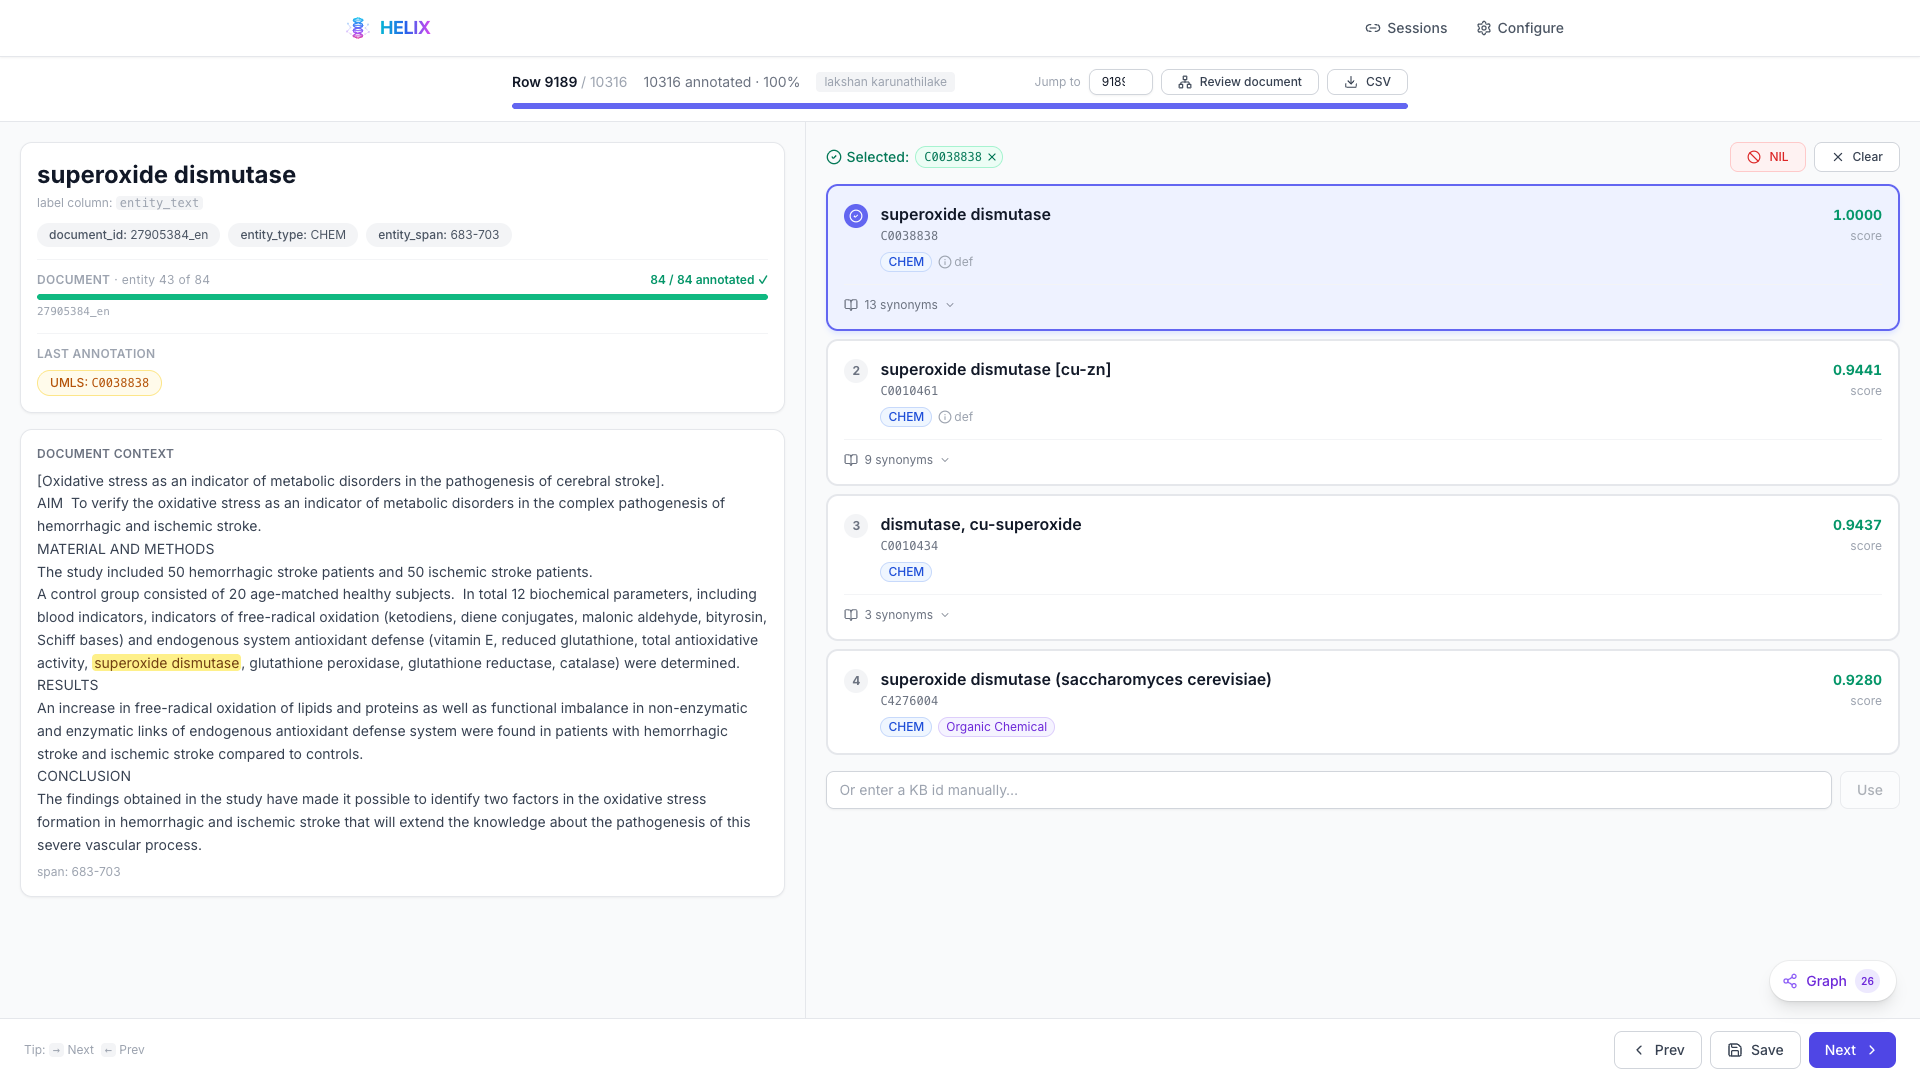
\includegraphics[width=0.92\textwidth]{figures/annotate.png}
\caption{HELIX annotation interface (individual level): the mention in its document
context (left) and the ranked candidate list with the auto-selected pick and
interruptible countdown, which the annotator confirms, overrides, or marks NIL (right).}
\label{fig:ui}
\end{figure}

\begin{figure}[t]
\centering
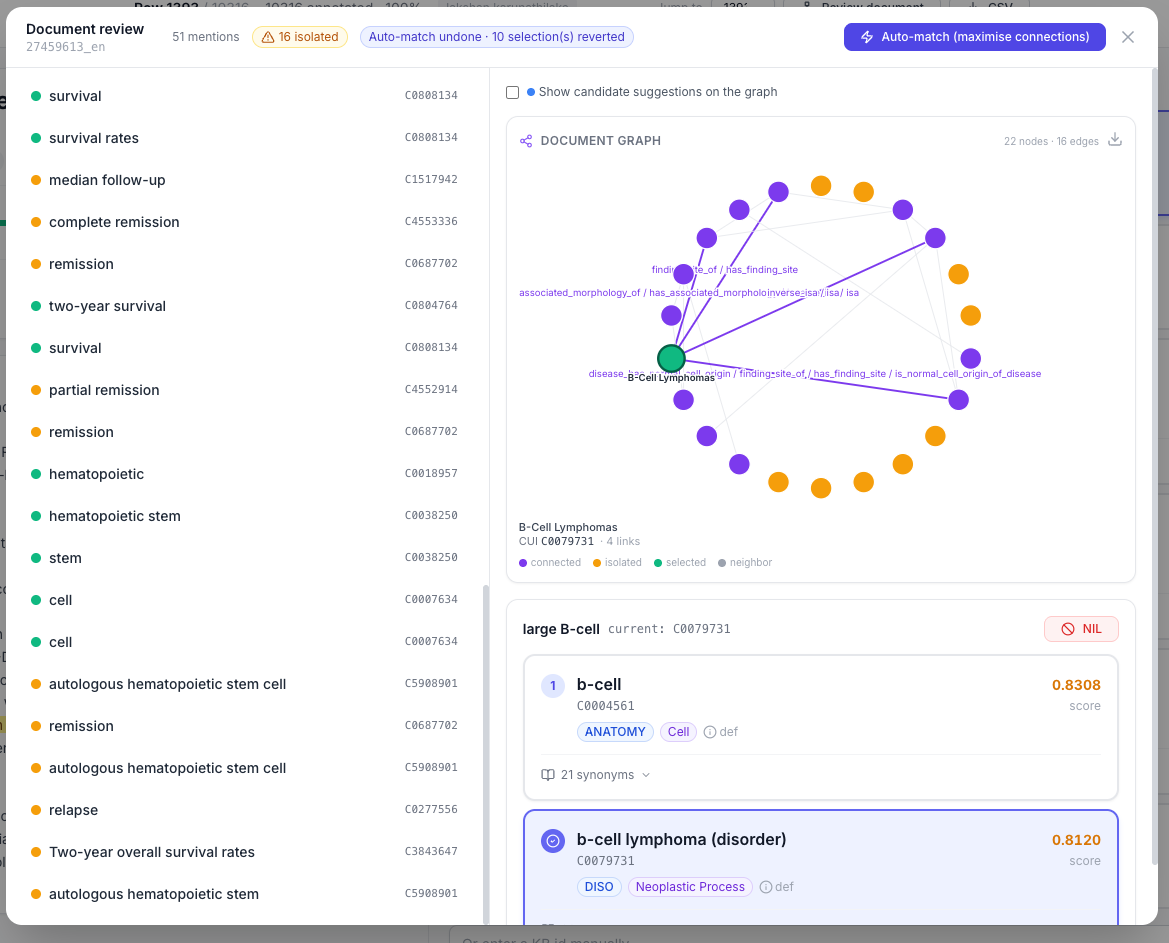
\includegraphics[width=0.80\textwidth]{figures/graph_panel.png}
\caption{Document-level graph review: accepted concepts form one subgraph with node
degrees shown and \emph{isolated} picks flagged; the annotator disambiguates by graph
context, and substituting a better-connected candidate rewrites the annotation and
re-computes coherence.}
\label{fig:docreview}
\end{figure}

% ==============================================================================
\section{Evaluation}
\label{sec:eval}

We evaluate the automatic pipeline against the already-annotated BC5CDR gold on
both the chemical and disease tracks: dense-retrieval accuracy, the effect of
dictionary index construction, the automatic graph connection-maximisation step
measured against gold, and a query-cost/latency profile. All numbers below are
measured with \texttt{eval/score.py} (any-match).

\subsection{Datasets and Metrics}
\label{sec:data}
We use three biomedical corpora (Table~\ref{tab:datasets}). \textbf{BC5CDR}~\cite{bc5cdr}
(chemical and disease tracks, MeSH, BioSyn preprocessing; SAPBERT$+$FAISS with a MeSH
adapter) is our primary retrieval and graph-cost corpus. \textbf{MedMentions
ST21pv}~\cite{mohan2019medmentions} ($203{,}282$ mentions, $21$ UMLS types) is
a large, fine-grained stress test that exposes the Acc@$k$--Acc@1 gap the graph step
targets. \textbf{BioNNE-R}~\cite{bionner} abstracts (UMLS) provide the document-level case
study of how alternative selections reveal different graph edges
(Sec.~\ref{sec:graphresults}). Our UMLS retrieval index and knowledge graph are both
built from the \textbf{UMLS 2025AA} release. As our focus is \emph{the graph edges a selection
reveals}, BC5CDR and BioNNE-R carry the graph analysis while MedMentions motivates it.

\begin{table}[t]
\caption{Evaluation datasets and their role. Mentions as train\,/\,dev\,/\,test
where applicable; KB = target knowledge base. BC5CDR and the BioNNE-R case study
drive the graph analysis; MedMentions establishes the retrieval gap.}
\label{tab:datasets}
\centering
\footnotesize
\resizebox{\columnwidth}{!}{%
\begin{tabular}{llll}
\toprule
Corpus & KB & Mentions & Role in this evaluation \\
\midrule
BC5CDR-chemical    & MeSH          & $5{,}203/5{,}347/5{,}385$ & dense retrieval; graph cost \& edges \\
BC5CDR-disease     & MeSH          & $4{,}182/4{,}244/4{,}424$ & dense retrieval; index-construction study \\
MedMentions ST21pv & UMLS 2025AA & $203{,}282$               & retrieval coverage; Acc@$k$--Acc@1 gap \\
BioNNE-R             & UMLS 2025AA   & -                  & document-level graph edge-reveal case study \\
\bottomrule
\end{tabular}%
}
\end{table}

We report \textbf{Acc@1} and \textbf{Acc@$k$} ($k{=}10$, the retrieval ceiling),
and for the graph step the nodes tackled, edges \emph{discovered}, and per-document
query latency (Sec.~\ref{sec:cost}). A prediction is correct under \emph{any-match}:
its identifier matches any of the mention's gold concepts.

\subsection{Retrieval Results}
Our experiments evaluate dense retrieval (SAPBERT$+$FAISS with a MeSH adapter);
automating the annotator's selection with an LLM re-ranker is out of scope here and
left to future work (Sec.~\ref{sec:future}).
Table~\ref{tab:results} is our overall results table: dense retrieval (Acc@10 and
Acc@1) together with Acc@1 after the graph gate across pin thresholds and the
\emph{ungated} ablation. Retrieval is strong on BC5CDR (in-dictionary; up to
$96\%$ full-corpus) and much lower on the open-vocabulary MedMentions/UMLS setting.

\begin{table}[t]
\caption{Overall results (\%, any-match). BC5CDR: full dev/train/test splits
($500$ docs each); MedMentions ST21pv: $400$-doc sample.
\emph{Acc@1}\,/\,\emph{Acc@10} = dense top-1\,/\,top-10; the $\tau_p$ columns give
Acc@1 after the graph gate (Alg.~\ref{alg:graph}, $\delta{=}0.1$), \emph{Ungated}
removes it. \emph{Index}: general/full = whole ontology (open-vocabulary),
gold = corpus-derived (in-dictionary). The gate holds Acc@1 across the sweep; only
ungated collapses it.}
\label{tab:results}
\centering
\setlength{\tabcolsep}{4pt}
\resizebox{\columnwidth}{!}{%
\begin{tabular}{lllcccccc}
\toprule
& & & & & \multicolumn{3}{c}{Graph gate ($\tau_p$)} & \\
\cmidrule(lr){6-8}
Corpus & Index & Split & Acc@10 & Acc@1 & $0.95$ & $0.85$ & $0.70$ & Ungated \\
\midrule
MedMentions ST21pv & UMLS, general & --    & 54.5 & 34.8 & 34.6 & 34.8 & 34.8 & 33.5 \\
MedMentions ST21pv & UMLS, gold    & --    & 98.7 & 69.9 & 69.9 & 69.9 & 69.9 & 50.4 \\
\midrule
BC5CDR-chemical & MeSH, full & dev   & 85.3 & 82.7 & 83.5 & 83.1 & 83.0 & 70.8 \\
                &            & train & 85.2 & 81.9 & 82.2 & 82.5 & 81.9 & 69.9 \\
                &            & test  & 81.6 & 78.6 & 78.6 & 78.7 & 78.7 & 66.7 \\
\addlinespace
                & MeSH, gold & dev   & 93.3 & 93.3 & 93.3 & 93.3 & 93.3 & 75.8 \\
                &            & train & 93.3 & 93.3 & 93.2 & 93.3 & 93.3 & 77.7 \\
                &            & test  & 86.7 & 85.7 & 85.6 & 85.7 & 85.7 & 70.6 \\
\midrule
BC5CDR-disease  & MeSH, full & dev   & 80.7 & 72.6 & 71.5 & 72.1 & 72.6 & 57.3 \\
                &            & train & 80.9 & 71.7 & 71.4 & 71.9 & 71.7 & 56.4 \\
                &            & test  & 81.9 & 72.6 & 72.2 & 72.8 & 72.5 & 59.0 \\
\addlinespace
                & MeSH, gold & dev   & 96.3 & 95.4 & 95.5 & 95.3 & 95.4 & 69.5 \\
                &            & train & 95.9 & 95.4 & 95.4 & 95.4 & 95.4 & 70.0 \\
                &            & test  & 90.7 & 87.5 & 86.5 & 87.1 & 87.4 & 64.9 \\
\bottomrule
\end{tabular}}
\end{table}

\paragraph{An in-dictionary ceiling.}
These BC5CDR figures should be read with care. The BioSyn dictionary is
\emph{derived from the corpus}, so the index is guaranteed to contain every gold
concept; the numbers are therefore a favourable \emph{in-dictionary} ceiling rather
than open-vocabulary accuracy, and part of the score reflects dictionary coverage
rather than encoder quality. Re-indexing the same corpus against the \emph{full}
MeSH ontology ($1$M concepts) makes this concrete: with the same encoder, Acc@1
falls from $93.3/95.4$ (chemical/disease gold, dev) to $82.7/72.6$
(Table~\ref{tab:results}). The realistic open-vocabulary regime is thus the
full-ontology setting --- most sharply our MedMentions/UMLS results
(Sec.~\ref{sec:medmentions}), where accuracy is far lower and coverage is the
binding constraint. The lesson: for dictionary EL, \emph{what is in the index} is a
first-order factor that must be reported alongside the retriever.

\subsection{Generalisation to UMLS: MedMentions ST21pv}
\label{sec:medmentions}
To test HELIX beyond MeSH, we link all $203{,}282$ MedMentions ST21pv mentions against
a general UMLS index. Overall dense Acc@1 is $34.5\%$ (Acc@10 $54.8\%$), far below
BC5CDR, because the ceiling is set by \emph{index coverage}: whole ST21pv semantic
types (e.g.\ Eukaryote, Population Group, Bacterium) are absent from the general index
and score near zero. Rebuilding the index around the ST21pv \emph{target} concepts
confirms this directly (Table~\ref{tab:results}): with the same encoder and mentions,
Acc@10 rises $54.8\rightarrow98.7\%$ and Acc@1 $34.5\rightarrow69.9\%$, and the
previously-absent types recover to $56$--$86\%$. The encoder is not the bottleneck;
retrieval quality is gated first by \emph{what is in the index}.

\subsection{Graph-Assisted Review}
\label{sec:graphresults}
The graph step does not improve retrieval; it targets the \emph{Acc@$k$--Acc@1
gap} (gold retrieved but not ranked first), which is substantial on hard corpora
($20.3$ points on MedMentions) and near-zero where retrieval is confident.
The graph columns of Table~\ref{tab:results} sweep the gate's pin threshold $\tau_p$
across all three corpora. Two findings emerge. First, \emph{the gate is safe}: across
the entire range $\tau_p\in[0.70,0.95]$ Acc@1 holds at the retrieval baseline on every
corpus, because confident picks are pinned and only near-ties can move --- the graph
never degrades a well-retrieved document. Second, \emph{the gate is essential}:
removing it (\emph{ungated}) collapses Acc@1 by $17.5$ points on BC5CDR-chemical
($93.3\rightarrow75.8$, dev), $25.9$ on BC5CDR-disease ($95.4\rightarrow69.5$), and $1.3$ on
MedMentions, as unconstrained edge maximisation overrides confident top-1 picks in
favour of hub concepts (on the MeSH graph $\sim$56\% of edges are structural, e.g.\
\texttt{sibling}). Automatic gains are small here --- BC5CDR's in-dictionary gap is
tiny and MedMentions is coverage-bound --- so the gate's role is protective; the
feature's primary value is \emph{interactive}: the graph maximises document-level
knowledge for a human who accepts or overrides on the same view.

\paragraph{Worked example (BioNNE-R): the graph reveals knowledge, but degree is not
correctness.}
Re-binding a mention changes the relations that connect it to the rest of the
document (Fig.~\ref{fig:docsub}). Often the \emph{correct} reading is the
better-connected one: for a ``skin'' mention, the general anatomical concept
\emph{Skin} lights up a rich neighbourhood (\texttt{finding\_site\_of}/%
\texttt{has\_finding\_site}, \texttt{has\_location}/\texttt{location\_of},
\texttt{specimen\_source\_topography}) while the narrower \emph{Skin, Human} attaches
almost nothing (a--b) --- the graph surfaces document structure the flat cards hide
and points to the coherent choice. But connectivity is \emph{not} a proxy for
correctness: for an ``oxidation'' mention, \emph{Oxidation-Reduction} reveals
\emph{more} edges (\texttt{biological\_process\_involves\_gene\_product}, \texttt{isa},
\ldots) than the plainer \emph{Oxidation} (c--d), yet the more-connected concept is
the wrong annotation here. Hub-like concepts out-link specific ones, so the choice
must be read from the \emph{relations and context}, not degree alone --- the
qualitative face of the ungated ablation (Table~\ref{tab:results}) and why HELIX gates
on confidence and leaves the call to the annotator.

\begin{figure}[t]
\centering
\begin{minipage}[t]{0.49\textwidth}\centering
  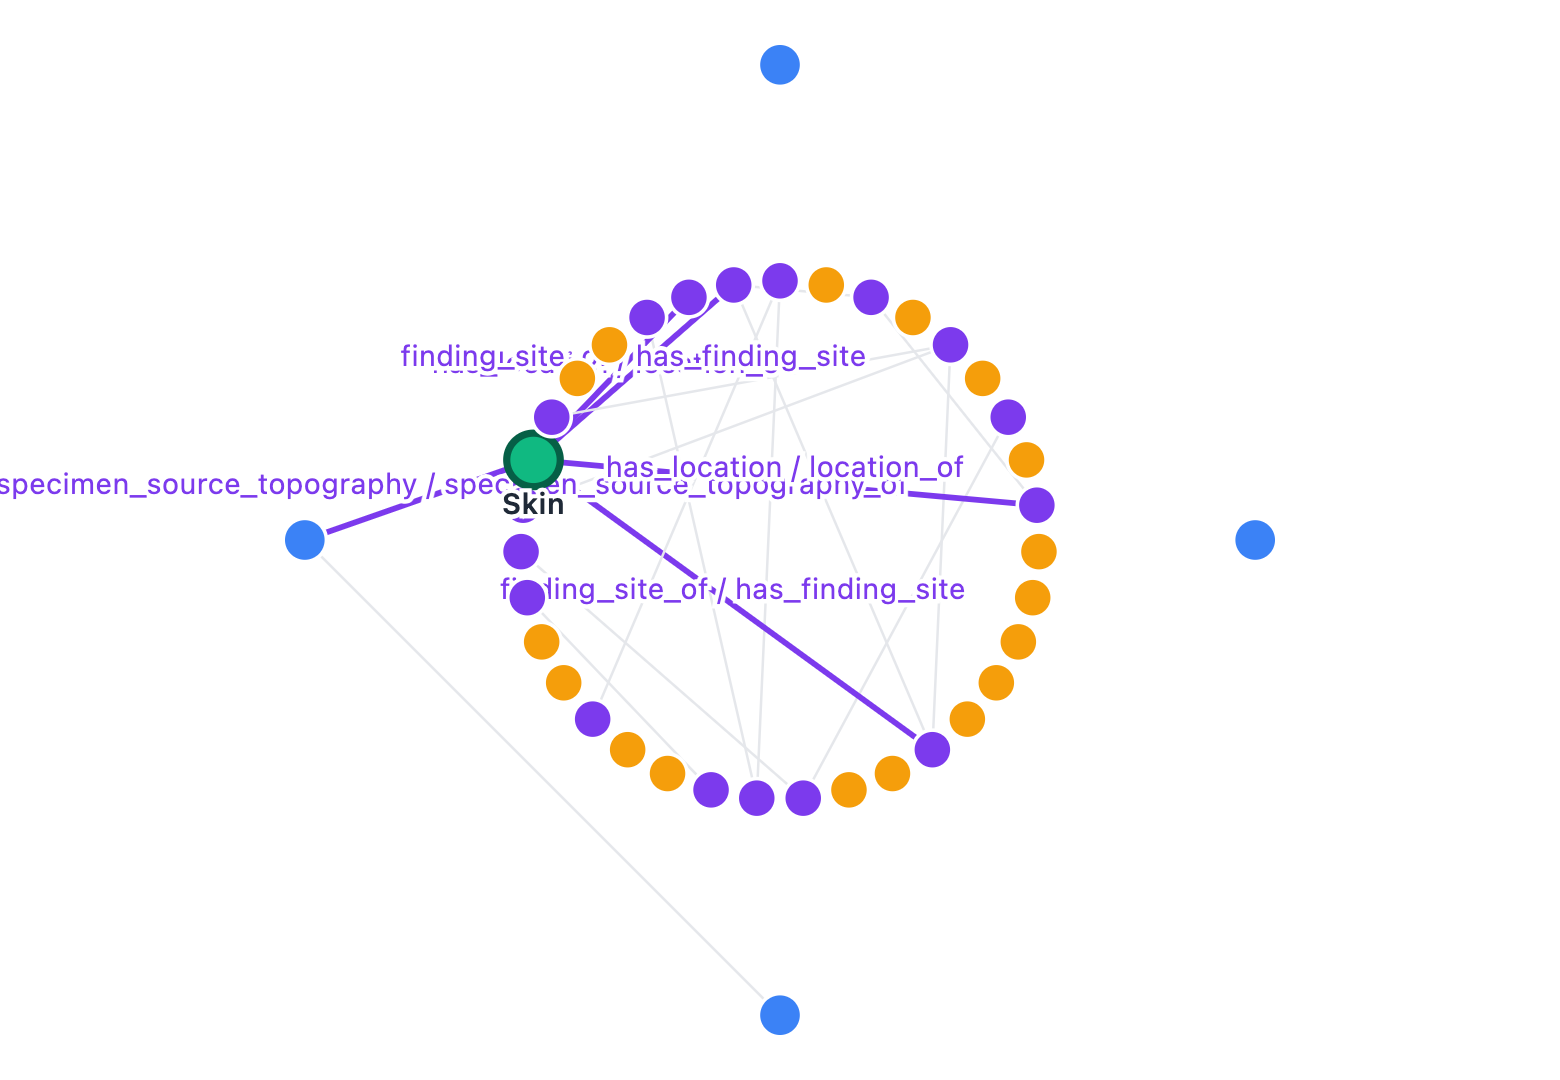
\includegraphics[width=\linewidth]{figures/sub_skin.png}\\
  {\footnotesize (a) \emph{Skin} --- correct, richly connected}
\end{minipage}\hfill
\begin{minipage}[t]{0.49\textwidth}\centering
  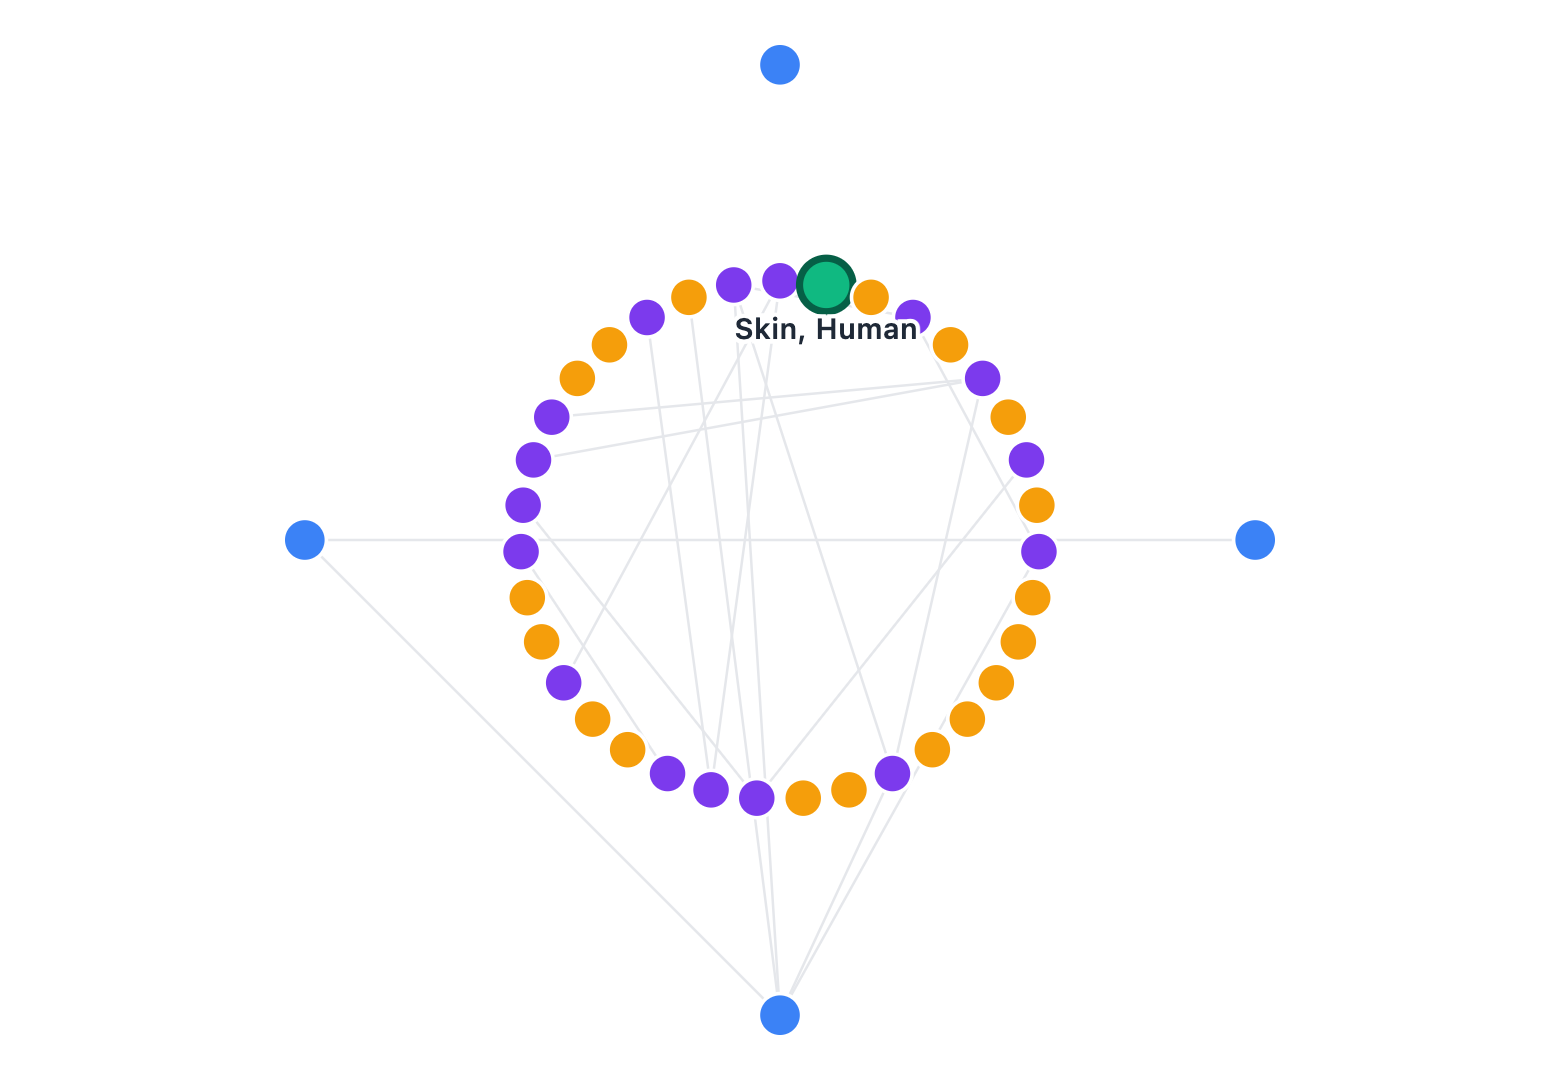
\includegraphics[width=\linewidth]{figures/sub_skin_human.png}\\
  {\footnotesize (b) \emph{Skin, Human} --- few links}
\end{minipage}

\vspace{4pt}

\begin{minipage}[t]{0.49\textwidth}\centering
  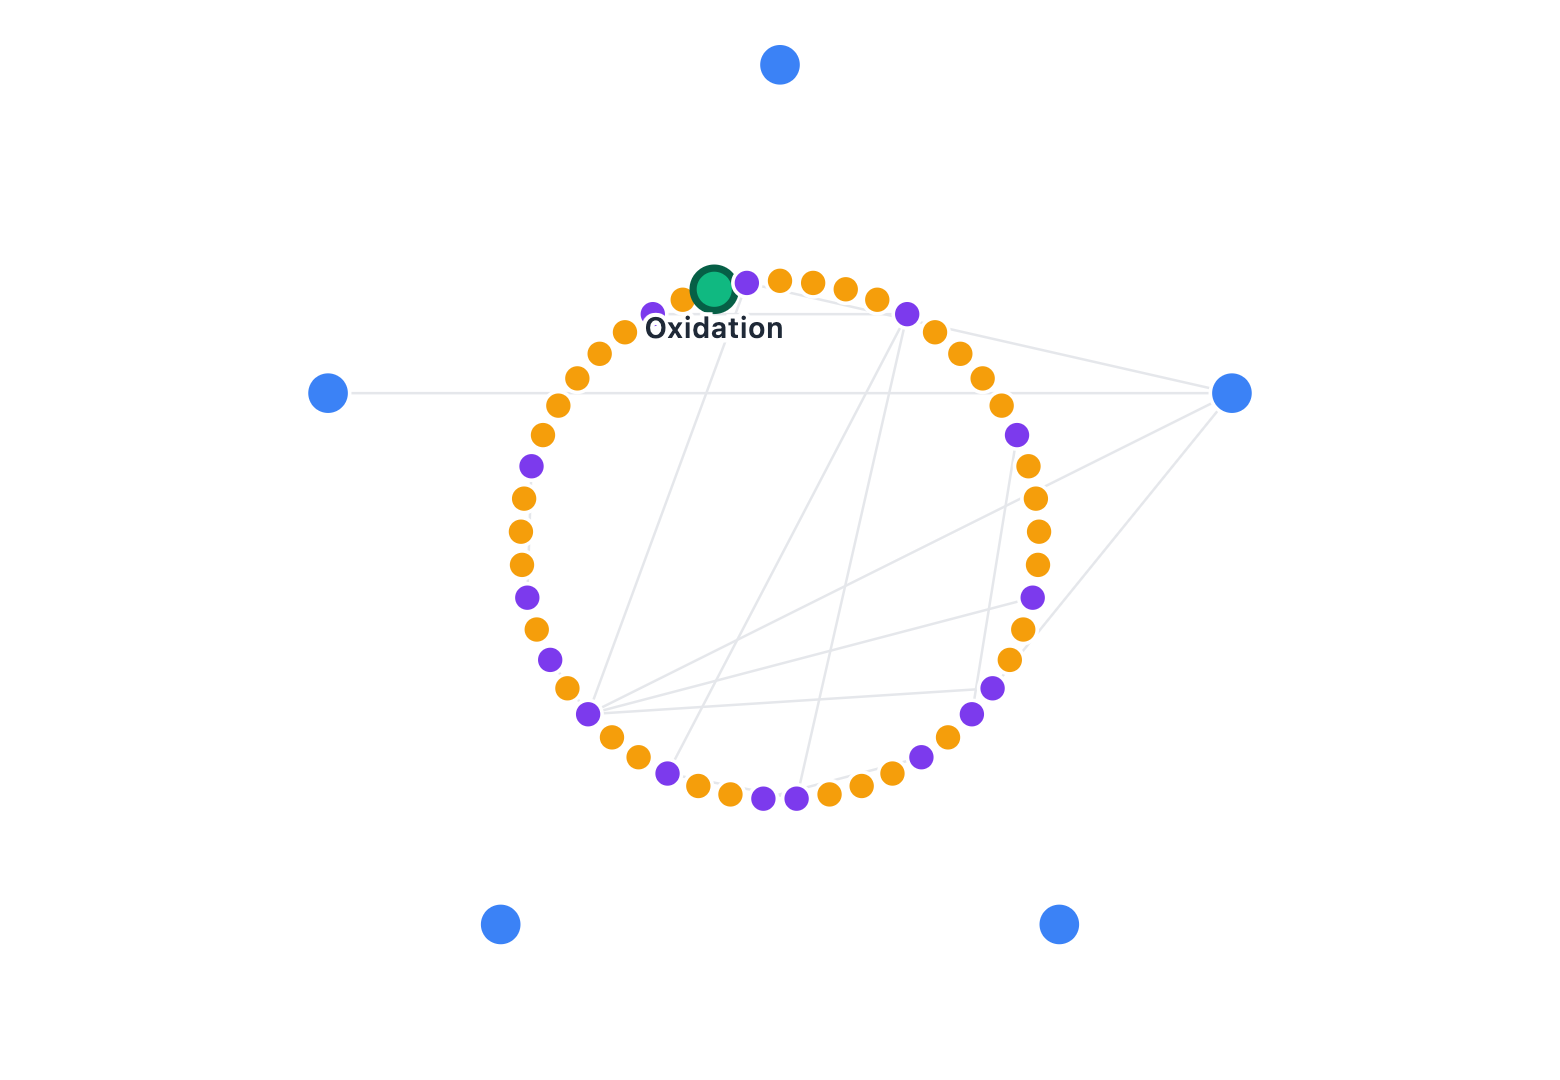
\includegraphics[width=\linewidth]{figures/sub_oxred.png}\\
  {\footnotesize (c) \emph{Oxidation-Reduction} --- more links, but wrong}
\end{minipage}\hfill
\begin{minipage}[t]{0.49\textwidth}\centering
  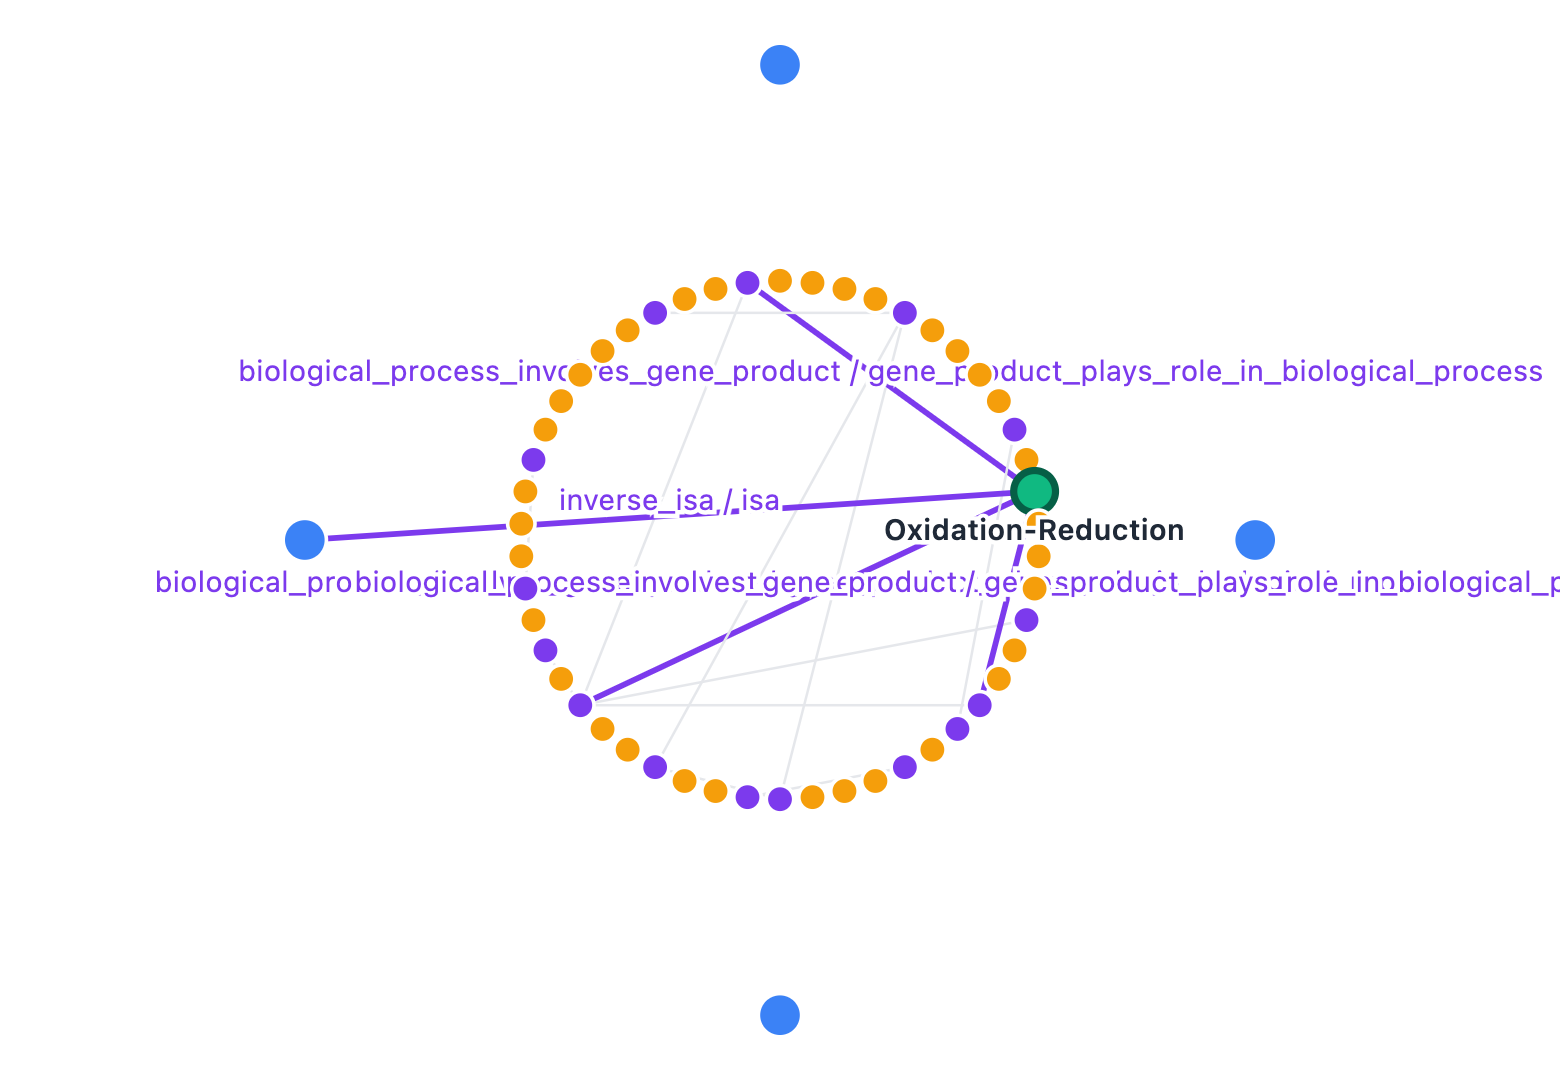
\includegraphics[width=\linewidth]{figures/sub_oxidation.png}\\
  {\footnotesize (d) \emph{Oxidation} --- the correct annotation}
\end{minipage}
\caption{Document-level substitution on BioNNE-R. \textbf{(a--b)} The better-connected
concept is right: \emph{Skin} reveals many relations where \emph{Skin, Human} reveals
almost none. \textbf{(c--d)} But more is \emph{not} always right:
\emph{Oxidation-Reduction} out-links the correct \emph{Oxidation}. Degree helps but is
not a correctness signal --- the pick must be read from relations and context. Green:
selected; blue: alternative; violet/orange: connected/isolated accepted concepts.}
\label{fig:docsub}
\end{figure}

% ------------------------------------------------------------------------------
\subsection{Query Cost and Latency}
\label{sec:cost}

HELIX stays interactive end-to-end: dense retrieval is $\sim$16\,ms per mention
(p95 $17$) and the full candidate request $\sim$17\,ms; document writes are a single
in-memory pass. The document-level step's cost is one Neo4j edge query, which we
profile across all three corpora (Fig.~\ref{fig:graphcost}). Latency tracks
\emph{edge discovery} over the candidate set more than raw node count, and grows
near-linearly with the number of candidate nodes tackled per document: BC5CDR's small
MeSH subgraphs ($16$--$25$ nodes/doc) cost $\sim$5\,ms on average (p95 $\le13$),
while MedMentions' larger UMLS subgraphs ($\sim$150 nodes/doc, up to $\sim$290) reach
$18$\,ms mean (p95 $40$) --- always within interactive range.

\begin{figure}[t]
\centering
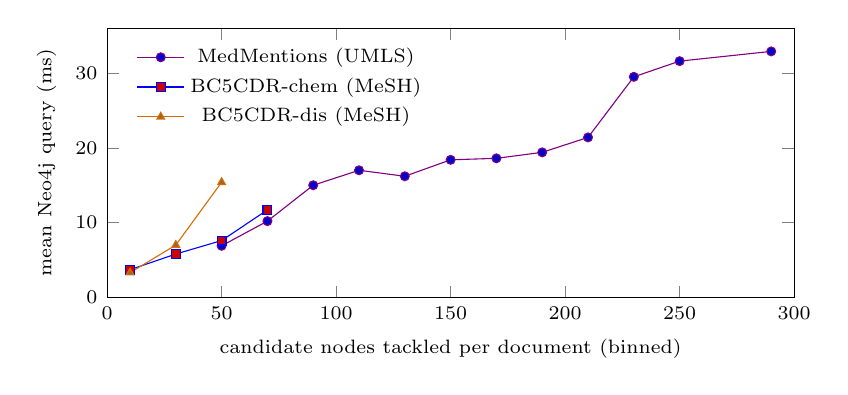
\begin{tikzpicture}
\begin{axis}[
  width=0.85\textwidth,height=5cm,
  xlabel={candidate nodes tackled per document (binned)},
  ylabel={mean Neo4j query (ms)},
  xmin=0,xmax=300,ymin=0,ymax=36,
  legend pos=north west,legend style={font=\scriptsize,draw=none,fill=none},
  tick label style={font=\scriptsize},label style={font=\scriptsize},
  mark size=1.6pt,
]
\addplot+[mark=*,color=violet] coordinates {
  (50,6.9) (70,10.2) (90,15.0) (110,17.0) (130,16.2) (150,18.4) (170,18.6)
  (190,19.4) (210,21.4) (230,29.5) (250,31.6) (290,32.9)};
\addplot+[mark=square*,color=blue] coordinates {(10,3.7) (30,5.8) (50,7.6) (70,11.7)};
\addplot+[mark=triangle*,color=orange!85!black] coordinates {(10,3.3) (30,7.0) (50,15.4)};
\legend{MedMentions (UMLS), BC5CDR-chem (MeSH), BC5CDR-dis (MeSH)}
\end{axis}
\end{tikzpicture}
\caption{Graph edge-query latency vs.\ candidate nodes per document, across all three
corpora (binned, dev-split samples). Cost grows near-linearly and stays interactive
($\le\!35$\,ms); edge discovery, not node lookup, dominates.}
\label{fig:graphcost}
\end{figure}

% ==============================================================================
\section{Discussion and Limitations}
\label{sec:discussion}

HELIX is deliberately positioned as \emph{assistive}: the graph component
informs a human decision rather than replacing it, and the document-level step is a
human-driven analogue of collective disambiguation rather than automatic
inference. This design keeps annotations auditable---every suggestion, override,
and renegotiation is logged---which matters for downstream KG construction.

Several limitations apply. First, our evaluation exercises dense retrieval and the
graph step; automating the annotator's selection with an LLM is left to future work
(see below). Second, our BC5CDR figures are a corpus-derived \emph{in-dictionary}
ceiling rather than open-vocabulary accuracy (the BioSyn dictionary is derived from
the corpus, so it contains every gold concept); the realistic open-vocabulary regime
is the MedMentions/UMLS setting, where accuracy is far lower and dictionary coverage
is the binding constraint. Third, \emph{ungated} edge
maximisation over-corrects (Table~\ref{tab:results}); HELIX's confidence-gated
algorithm (Algorithm~\ref{alg:graph}) prevents this by construction --- pinning
confident picks and re-ranking only near-ties --- and its large-scale evaluation
against gold is ongoing. The graph's primary value is \emph{interactive}:
maximising document-level knowledge for a human who can accept or override every
decision. Finally, our study uses a single annotator, so we do not report
inter-annotator agreement.

\subsection{Future Work}
\label{sec:future}
Several directions follow directly. (1)~\textbf{Automating the annotator's selection
(LLM).} The natural next step is to automate the decision the human now makes: a
grounded, retrieval-augmented LLM re-ranker that---constrained to the retrieved
candidate set (and optionally the graph neighbourhood) via a strict enumerated
schema---proposes the selection for the annotator to confirm or override. Studying
its accuracy/cost/latency trade-off, and how much of the human's effort it can
safely absorb, is future work.
(2)~\textbf{Confidence-gated graph, at scale.} Algorithm~\ref{alg:graph} is
implemented; evaluating it against gold across more corpora, tuning $\tau_p$ and
$\delta$, and restricting the graph to semantic (non-structural) relations is
ongoing. (3)~\textbf{Open-vocabulary retrieval.} Moving beyond corpus-derived
dictionaries to full-ontology indexes (as in our MedMentions/UMLS setting), where
coverage is the binding constraint.
(4)~\textbf{User study.} A multi-annotator study reporting inter-annotator
agreement, acceptance/override rates, and NASA-TLX workload. We do not pursue
lexical/hybrid retrieval further: in our tests an auxiliary BM25\,$+$\,$n$-gram
strand fused with the dense list did not help on BC5CDR (the domain-adapted encoder
already handles short mentions), so we retain dense retrieval alone.

% ==============================================================================
\section{Conclusion}
\label{sec:conclusion}

We presented HELIX, an expert-in-the-loop biomedical entity-linking annotation
tool that combines dense retrieval with a two-level graph-aware review
process---candidate-neighbourhood disambiguation and a document-level
coherence-negotiation view. HELIX targets two concrete
pain points in EL curation: flat candidate presentation and incoherent
per-mention decisions. On BC5CDR, dense retrieval
reaches up to $96\%$ Acc@1; on the far larger MedMentions ST21pv (UMLS) it reaches
$34.5\%$, and across both corpora we show that dictionary index
\emph{construction and coverage} dominate retrieval quality (a $20$-point swing on
BC5CDR; whole semantic types near-zero on MedMentions when absent from the index).
We further show the graph step is inexpensive ($9.4$\,ms mean per document) but
must be confidence-gated to help rather than over-correct. We release the system,
its configuration, and an evaluation harness
to support scalable entity-linking annotation.

% ---- Bibliography ----
\bibliographystyle{splncs04}
\bibliography{references}

\end{document}
